\RequirePackage{luatex85}
\documentclass[tikz]{standalone}
\usepackage{tikz, tkz-euclide}
\usetkzobj{all} %% PROVIDES \tkzMarkRightAngle REQUIRES tkz-euclide

\begin{document}
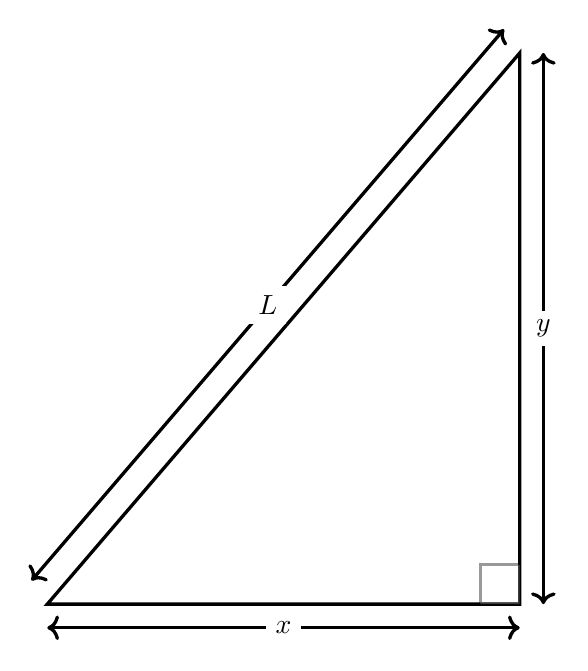
\begin{tikzpicture}[very thick]
\coordinate (A) at (0,0);
\coordinate (O) at (6,0);
\coordinate (B) at (6,7);
\draw (A)--(O)--(B)--cycle;
\draw[<->, yshift=-0.3cm] (0,0) -- node[fill, white]{\color{black}$x$} (6,0);
\draw[<->, xshift=0.3cm] (6,0) -- node[fill, white]{\color{black}$y$} (6,7);
\draw[<->, shift={(-0.2,0.3)}] (0,0) -- node[fill, white]{\color{black}$L$} (6,7);
\tkzMarkRightAngle[fill=white,size=0.5,opacity=.4](A,O,B)
\end{tikzpicture}

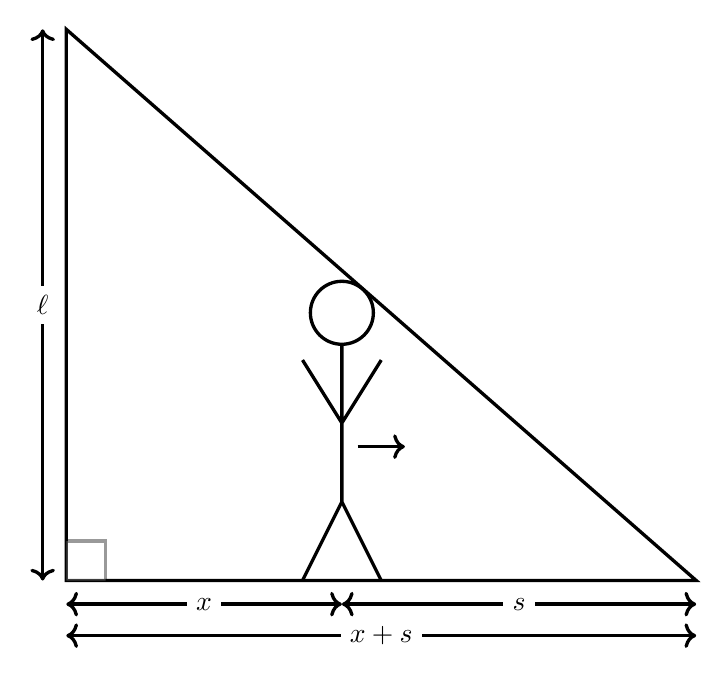
\begin{tikzpicture}[very thick]
\coordinate (B) at (0,7);
\coordinate (O) at (0,0);
\coordinate (A) at (8,0);
\draw (B)--(O)--(A)--cycle;
\draw[<->, xshift=-0.3cm] (0,7) -- node[fill, white]{\color{black}$\ell$} (0,0);
\draw[<->, yshift=-0.7cm] (0,0) -- node[fill, white]{\color{black}$x+s$} (8,0);
\draw[<->, yshift=-0.3cm] (0,0) -- node[fill, white]{\color{black}$x$} (3.5,0);
\draw[<->, yshift=-0.3cm] (3.5,0) -- node[fill, white]{\color{black}$s$} (8,0);
\tkzMarkRightAngle[fill=white,size=0.5,opacity=.4](A,O,B)
\draw[very thick] (3.5, 1) -- (3.5, 3) (3, 0) -- (3.5, 1) (4, 0) -- (3.5, 1) (3.5, 2) -- (4, 2.8) (3.5, 2) -- (3, 2.8) (3.7, 1.7) edge[->] (4.3, 1.7) (3.5,3.4) circle (0.4cm); % stickman
\end{tikzpicture}

\begin{tikzpicture}
\draw[->] (-2.5,0) -- (4,0) node[below] {$x$};
\draw[->] (0,-1) -- (0,4) node[left] {$y$};
\draw[domain=0:3, very thick] plot (\x, \x*\x/3);
\draw (0,0) -- (3,3);
\fill (0,0) circle (2pt) (3,3) circle (2pt);
\draw (0,0) node[below left]{Origin (0,0)};
\draw (3,3) node[right]{$(x,y) = (x,x^2)$};
\draw[<-] (3,3) ++(-0.1,0.1) -- ++(-0.5,0.5) node[above, inner sep=0]{$y=x^2$};
\end{tikzpicture}
\end{document}